We now present an RTS game we used as a case study, created with Casanova, and the benchmarks that test the action implementation. In the game players must conquer a star system made up of various planets. Each planet builds fleets which are used to fight the fleets of the other players and to conquer more planets. A planet is conquered when a fleet of a player is near it and no other enemy fleet is defending it.

\subsection{Case study}

Three actions are required in this game: The first action, called \texttt{Fight Action}, defines how a fleet fights enemy fleets in range. The fight action subtracts $0.5 \cdot dt$ \texttt{life} points from the in-range enemy fleet during every frame (action tick).

\begin{lstlisting}[language=Caml]
Fleet = {Position: Rule Vector2;FightAction: FightAction;Owner: Ref Player;Life: Var float32;Fight: FightAction }
\end{lstlisting}

The Fight Action is defined as follows:

\begin{lstlisting}[language=sql]
FightAction = TARGET Fleet; RESTRICTION Owner <> Owner; RADIUS 150.0; TRANSFER CONSTANT Life - 0.5;
\end{lstlisting}

The target is an entity of which the type is \textbf{Fleet}. The condition to execute the action is that the fleet must be an enemy (i.e., not the player). The \texttt{attack range} is 150 units of distance. 0.5 \texttt{life} points are subtracted for every attack.

The second action is called \texttt{BuildAction}. It allows a planet to create a ship. In order to build a ship, a planet must gather 10 mineral units. Each planet has a field called \texttt{GatherSpeed} which determines how fast it gathers minerals. Every tick the planet's mineral stash is increased by this amount. This action is a threshold action where the threshold value is the minerals of the planet. As soon as the threshold value is reached, we set the field \texttt{NewFleet} to TRUE (it is used by the engine to create a new fleet), and \texttt{Minerals} to 0 to reset the counter. The planet and its actions are:

\begin{lstlisting}[language=Caml]
Planet = {Position: Vector2;Owner: Rule Ref Player;NewFleet: Rule bool;BuildAction:BuildAction;EnemyOrbitingFleetsAction : EnemyOrbitingFleetsAction;GatherSpeed: float32;Minerals: Var float32 }
\end{lstlisting}

\begin{lstlisting}[language=sql]
BuildAction =
TARGET Self; TRANSFER CONSTANT Minerals + GatherSpeed; THRESHOLD Minerals 10.0; OUTPUT NewFleet := true; OUTPUT Minerals := 0.0
\end{lstlisting}

A Casanova rule is appointed to read the value of NewFleet and, when it is true, to spawn a new fleet.

The third action is required to check if a planet can be conquered by a fleet. A fleet can conquer a planet if there is no enemy fleet near it and if it is sufficiently close. Thus the action definition is the following:

\begin{lstlisting}[language=sql]
EnemyOrbitingFleetsAction =
TARGET Fleet; RESTRICTION Owner Not Eq Owner; RADIUS 25.0; INSERT Owner -> EnemyOrbitingFleets
\end{lstlisting}

The action will add an enemy fleet close enough to change the owner of the planet.

%Even the concept of drawing lasers can be implemented using the INSERT clause simply adding it to \texttt{FightAction} which inserts in a list all the targeted ships positions. In this way we can draw a laser from the source position to the target position. We omit this aspect for brevity.

\subsection{Evaluation}

We evaluated the performance of our approach with the case study, and two extra examples: an asteroid shooter, and an expanded version of the case study with more complex rules. All were implemented in Casanova. Table \ref{tab:code_length} shows a code length comparison between the REA implementation and standard Casanova rules for all three.

We note that in games with basic dynamics the code saving is low, due to the fact that there are few repeated patterns. The advantage of using REA becomes evident in a game with actions involving many types of targets, such as the expanded case study. Furthermore, we managed to drastically increase the performance of the game logic: as Figure \ref{fps_chart} shows, using REA (labeled ``with actions'') results in a speedup factor of 6 to 25, due to automated optimizations in the query evaluation. We also note that our implementation is flexible and general since it is possible to use actions to express a behaviour, such as a projectile collision, which is outside the domain of RTS games and traditional resource-based systems.

\begin{table}
\centering
\caption{CS (case study), Asteroid Shooter and Expanded CS code length}
\label{tab:code_length}
\begin{tabular}
{|l|c|c|c|c|c|c|}
\hline
& Game Entities & Rules & Actions & Total\\
\hline
\textit{CS with REA} & 41 & 71 & 19 & 131\\
\hline
\textit{CS without REA} & 40 & 90 & 0 & 130\\
\hline
\textit{Asteroid shooter with REA} & 33 & 33 & 6 & 72\\
\hline
\textit{Asteroid Shooter without REA} & 34 & 44 & 0 & 78\\
\hline
\textit{Extended CS with REA} & 135 & 138 & 40 & 313\\
\hline
\textit{Extended CS without REA} & 135 & 328 & 0 & 463\\
\hline
\end{tabular}
\end{table}
\begin{figure}
\centering
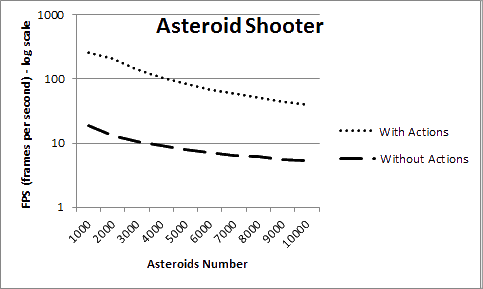
\includegraphics[scale=0.7]{Shooter.png}
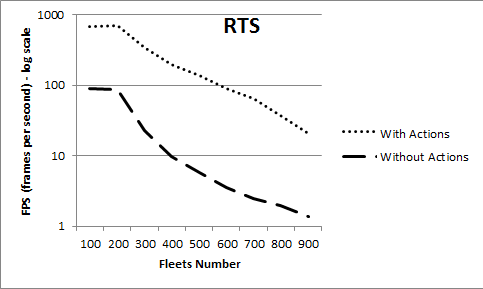
\includegraphics[scale=0.7]{RTS.png}
\caption{Frame rate as a function of numbers of entities.}
\label{fps_chart}
\end{figure} 